% 基礎数学 第02回 変数と関数・三角関数（CC BY-SA 4.0）
\documentclass[aspectratio=169]{beamer}
\usepackage{lfs-slides}
\lfscourse{基礎数学}

\title{変数と関数・三角関数}
\subtitle{基礎数学 第02回}
\author{}
\date{}

\begin{document}

\begin{frame}
  \titlepage
\end{frame}

\begin{frame}{今日のねらい}
  \lfsmessage{三角関数 ＝ 円をまわる点の座標}
  \bigskip
  \begin{itemize}
    \item 関数の考え方を確認する
    \item 角度を「弧の長さ」で測る（弧度法）
    \item 単位円で $\sin$，$\cos$，$\tan$ を定義する
    \item グラフ・周期・振幅を読み取る
    \item 工学では：振動・交流・ロボットの腕
  \end{itemize}
\end{frame}

\section{関数}

\begin{frame}{関数：入れると、1つに決まって出てくる}
  \begin{center}
    \begin{tikzpicture}
      \node[draw,rounded corners,minimum width=3cm,minimum height=1.2cm,fill=blue!8] (f) at (0,0) {関数 $f$};
      \node (in) at (-4,0) {入力 $x$};
      \node (out) at (4,0) {出力 $y = f(x)$};
      \draw[->,thick] (in) -- (f);
      \draw[->,thick] (f) -- (out);
    \end{tikzpicture}
  \end{center}
  \medskip
  例：$f(x) = 2x + 1$ のとき
  \[
    f(3) = 2 \cdot 3 + 1 = 7, \qquad f(-1) = 2 \cdot (-1) + 1 = -1
  \]
  \begin{block}{変数}
    $x$ のように、いろいろな値をとる文字を\textbf{変数}という
  \end{block}
\end{frame}

\section{弧度法}

\begin{frame}{弧度法：角度を「弧の長さ」で測る}
  \begin{columns}[c]
    \column{0.42\textwidth}
      \begin{center}
        % 弧度法：半径 1 の円で、角 θ に対する弧の長さが θ
\begin{tikzpicture}[scale=1.8]
  \draw[thin,gray] (0,0) circle (1);
  \draw[very thick] (0,0) -- (1,0) node[midway,below] {$1$};
  \draw[very thick] (0,0) -- (70:1);
  \draw[ultra thick,red] (1,0) arc (0:70:1);
  \node[red,right] at (35:1.05) {弧の長さ $\theta$};
  \draw (0.25,0) arc (0:70:0.25);
  \node at (35:0.4) {$\theta$};
  \fill (0,0) circle (1pt);
\end{tikzpicture}

      \end{center}
    \column{0.58\textwidth}
      半径 $1$ の円で、弧の長さが $\theta$ になる角を $\theta$（ラジアン）とする
      \medskip
      \begin{center}
        \renewcommand{\arraystretch}{1.3}
        \begin{tabular}{c|cccccc}
          度 & $30^\circ$ & $45^\circ$ & $60^\circ$ & $90^\circ$ & $180^\circ$ & $360^\circ$ \\ \hline
          弧度 & $\frac{\pi}{6}$ & $\frac{\pi}{4}$ & $\frac{\pi}{3}$ & $\frac{\pi}{2}$ & $\pi$ & $2\pi$
        \end{tabular}
      \end{center}
      \medskip
      \lfsmessage{$180^\circ = \pi$}
  \end{columns}
\end{frame}

\section{三角関数の定義}

\begin{frame}{単位円で定義する}
  \begin{columns}[c]
    \column{0.5\textwidth}
      \begin{center}
        % 単位円と三角関数の定義：P(cos θ, sin θ)
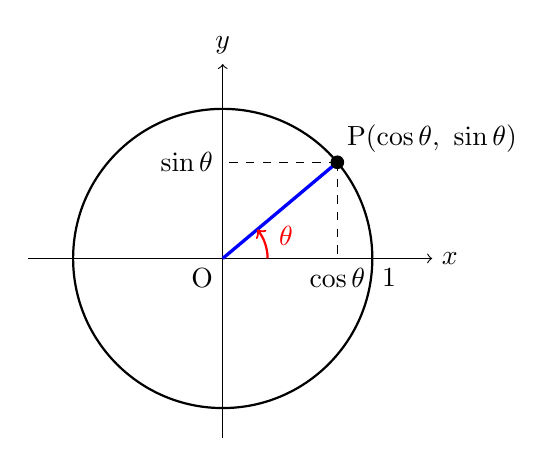
\begin{tikzpicture}[scale=1.9]
  \draw[->] (-1.3,0) -- (1.4,0) node[right] {$x$};
  \draw[->] (0,-1.2) -- (0,1.3) node[above] {$y$};
  \draw[thick] (0,0) circle (1);
  \coordinate (P) at (40:1);
  \draw[very thick,blue] (0,0) -- (P);
  \draw[dashed] (P) -- (P |- 0,0) node[below] {$\cos\theta$};
  \draw[dashed] (P) -- (0,0 |- P) node[left] {$\sin\theta$};
  \draw[->,red,thick] (0.3,0) arc (0:40:0.3);
  \node[red] at (20:0.45) {$\theta$};
  \fill (P) circle (1.3pt) node[above right] {$\mathrm{P}(\cos\theta,\ \sin\theta)$};
  \node[below left] at (0,0) {$\mathrm{O}$};
  \node[below right] at (1,0) {$1$};
\end{tikzpicture}

      \end{center}
    \column{0.5\textwidth}
      半径 $1$ の円（単位円）の上を、角 $\theta$ だけ回った点 P の
      \begin{itemize}
        \item $x$ 座標 ＝ $\cos\theta$
        \item $y$ 座標 ＝ $\sin\theta$
      \end{itemize}
      \[
        \tan\theta = \frac{\sin\theta}{\cos\theta}
      \]
      {\small 角が $90^\circ$ を超えても、負でも使える}
  \end{columns}
\end{frame}

\begin{frame}{よく使う値}
  \begin{center}
    \renewcommand{\arraystretch}{1.6}
    \begin{tabular}{c|ccccc}
      $\theta$ & $0$ & $\frac{\pi}{6}$ & $\frac{\pi}{4}$ & $\frac{\pi}{3}$ & $\frac{\pi}{2}$ \\ \hline
      $\sin\theta$ & $0$ & $\frac{1}{2}$ & $\frac{\sqrt{2}}{2}$ & $\frac{\sqrt{3}}{2}$ & $1$ \\
      $\cos\theta$ & $1$ & $\frac{\sqrt{3}}{2}$ & $\frac{\sqrt{2}}{2}$ & $\frac{1}{2}$ & $0$
    \end{tabular}
  \end{center}
  \medskip
  \begin{block}{覚え方}
    $\sin$ は右へ行くほど大きく、$\cos$ はその逆の順に並ぶ
  \end{block}
\end{frame}

\begin{frame}{$90^\circ$ を超える角：点 P の座標で読む}
  \begin{columns}[c]
    \column{0.44\textwidth}
      \begin{center}
        % 鈍角の例：θ = 3π/4（135°）の点 P(-√2/2, √2/2)。x 軸の負の側と 45° をなす直角三角形で値を読む
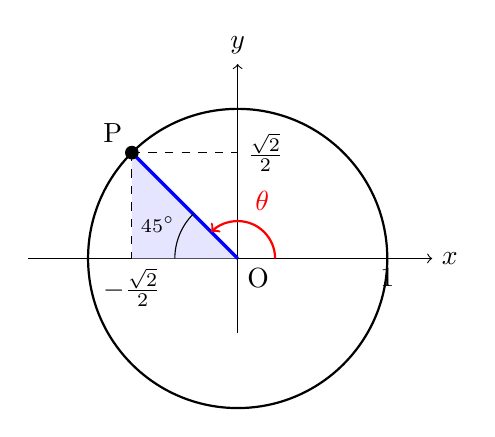
\begin{tikzpicture}[scale=1.9]
  \draw[->] (-1.4,0) -- (1.3,0) node[right] {$x$};
  \draw[->] (0,-0.5) -- (0,1.3) node[above] {$y$};
  \draw[thick] (0,0) circle (1);
  \coordinate (P) at (135:1);
  % 直角三角形（x 軸の負の側と 45°）
  \fill[blue!10] (0,0) -- (P) -- (P |- 0,0) -- cycle;
  \draw[very thick,blue] (0,0) -- (P);
  \draw[dashed] (P) -- (P |- 0,0) node[below] {$-\frac{\sqrt{2}}{2}$};
  \draw[dashed] (P) -- (0,0 |- P) node[right] {$\frac{\sqrt{2}}{2}$};
  % 角 θ = 135°（x 軸の正の向きから測る）
  \draw[->,red,thick] (0.25,0) arc (0:135:0.25);
  \node[red] at (67:0.42) {$\theta$};
  % 三角形の中の 45°
  \draw (-0.42,0) arc (180:135:0.42);
  \node[font=\scriptsize] at (157:0.58) {$45^\circ$};
  \fill (P) circle (1.3pt) node[above left] {$\mathrm{P}$};
  \node[below right] at (0,0) {$\mathrm{O}$};
  \node[below] at (1,0) {$1$};
\end{tikzpicture}

      \end{center}
    \column{0.56\textwidth}
      \lfsmessage{符号は P の位置で決まる}
      例：$\theta = \dfrac{3}{4}\pi$（$135^\circ$）
      \begin{itemize}
        \item 大きさ：P は $x$ 軸の負の側と $45^\circ$ をなす
        \item 符号：P は左上 → $x$ 座標は負、$y$ 座標は正
      \end{itemize}
      \[
        \sin\tfrac{3}{4}\pi = \tfrac{\sqrt{2}}{2}, \qquad
        \cos\tfrac{3}{4}\pi = -\tfrac{\sqrt{2}}{2}
      \]
      {\small $\theta = \pi$ なら P$(-1,\ 0)$ なので $\cos\pi = -1$、$\sin\pi = 0$}
  \end{columns}
\end{frame}

\begin{frame}{基本的な性質}
  \begin{columns}[t]
    \column{0.5\textwidth}
      \begin{block}{三平方の定理から}
        \[
          \sin^2\theta + \cos^2\theta = 1
        \]
        {\small 点 P は半径 $1$ の円の上にある}
      \end{block}
    \column{0.5\textwidth}
      \begin{block}{1周すると元に戻る}
        \[
          \sin(\theta + 2\pi) = \sin\theta
        \]
        \[
          \cos(\theta + 2\pi) = \cos\theta
        \]
      \end{block}
  \end{columns}
  \medskip
  例：$\sin\theta = \frac{3}{5}$\ （$0 < \theta < \frac{\pi}{2}$）なら
  $\cos\theta = \sqrt{1 - \frac{9}{25}} = \frac{4}{5}$
\end{frame}

\section{グラフ}

\begin{frame}{グラフ：波の形}
  \begin{center}
    % y = sin x と y = cos x のグラフ（0 ≦ x ≦ 2π）
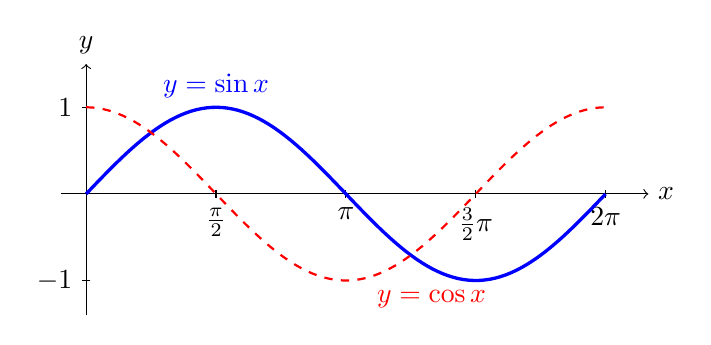
\begin{tikzpicture}[xscale=1.05,yscale=1.1]
  \draw[->] (-0.3,0) -- (6.8,0) node[right] {$x$};
  \draw[->] (0,-1.4) -- (0,1.5) node[above] {$y$};
  \foreach \x/\l in {1.5708/\frac{\pi}{2}, 3.1416/\pi, 4.7124/\frac{3}{2}\pi, 6.2832/2\pi}
    \draw (\x,0.05) -- (\x,-0.05) node[below] {$\l$};
  \draw (0.05,1) -- (-0.05,1) node[left] {$1$};
  \draw (0.05,-1) -- (-0.05,-1) node[left] {$-1$};
  \draw[very thick,blue,domain=0:6.2832,samples=100] plot (\x,{sin(\x r)});
  \draw[thick,red,dashed,domain=0:6.2832,samples=100] plot (\x,{cos(\x r)});
  \node[blue,above] at (1.5708,1) {$y=\sin x$};
  \node[red,below right] at (3.4,-1) {$y=\cos x$};
\end{tikzpicture}

  \end{center}
  \lfsmessage{$2\pi$ ごとに同じ形をくり返す（周期 $2\pi$）}
\end{frame}

\begin{frame}{振幅と周期}
  \[
    y = A \sin \omega x
  \]
  \begin{itemize}
    \item \textbf{振幅} $A$：波の高さ（$-A$ から $A$ まで動く）
    \item \textbf{周期} $\dfrac{2\pi}{\omega}$：1回分の波の長さ
  \end{itemize}
  \medskip
  例：$y = 2\sin 3x$ \ → \ 振幅 $2$，\ 周期 $\dfrac{2\pi}{3}$
\end{frame}

\section{工学では}

\begin{frame}{振動と交流}
  \lfsmessage{くり返す現象は $\sin$ で表す}
  \medskip
  \begin{itemize}
    \item 家庭のコンセントの電圧：1秒間に $50$ 回（地域によって $60$ 回）同じ変化をくり返す（$50$ Hz）
      \[
        V(t) = V_0 \sin(2\pi \cdot 50\, t) \qquad \text{（周期 } \tfrac{1}{50} \text{ 秒）}
      \]
    \item 音・ばねの振動・電波なども同じ形の式で表せる
  \end{itemize}
\end{frame}

\begin{frame}{ロボットの腕の先はどこ？}
  \begin{columns}[c]
    \column{0.5\textwidth}
      \begin{center}
        % ロボットアームの先端の位置：(L cos θ, L sin θ)
\begin{tikzpicture}[scale=1.5]
  \draw[->] (-0.3,0) -- (2.4,0) node[right] {$x$};
  \draw[->] (0,-0.3) -- (0,1.9) node[above] {$y$};
  \fill[gray!60] (-0.15,-0.15) rectangle (0.15,0);
  \draw[line width=5pt,orange!80!black,line cap=round] (0,0) -- (35:2);
  \fill (0,0) circle (2pt);
  \fill (35:2) circle (2pt);
  \node[above] at (35:2) {先端};
  \node[above left] at (35:1) {$L$};
  \draw (0.45,0) arc (0:35:0.45);
  \node at (17:0.65) {$\theta$};
  \draw[dashed] (35:2) -- ({2*cos(35)},0) node[below] {$L\cos\theta$};
  \draw[dashed] (35:2) -- (0,{2*sin(35)}) node[left] {$L\sin\theta$};
\end{tikzpicture}

      \end{center}
    \column{0.5\textwidth}
      長さ $L$ の腕を角 $\theta$ だけ持ち上げると、先端の位置は
      \[
        (L\cos\theta,\ L\sin\theta)
      \]
      例：$L = 2$，$\theta = \frac{\pi}{3}$ なら
      \[
        (2 \cdot \tfrac{1}{2},\ 2 \cdot \tfrac{\sqrt{3}}{2}) = (1,\ \sqrt{3})
      \]
  \end{columns}
\end{frame}

\begin{frame}{まとめ}
  \begin{itemize}
    \item 関数：入力 $x$ に対して出力 $f(x)$ が1つに決まる
    \item 弧度法：$180^\circ = \pi$
    \item 単位円上の点 P$(\cos\theta,\ \sin\theta)$，\ $\tan\theta = \dfrac{\sin\theta}{\cos\theta}$
    \item $\sin^2\theta + \cos^2\theta = 1$，\ 周期 $2\pi$
    \item $y = A\sin\omega x$：振幅 $A$，周期 $\dfrac{2\pi}{\omega}$
  \end{itemize}
  \bigskip
  \lfsmessage{次回：指数関数}
\end{frame}

\end{document}
